\documentclass[border=10pt]{standalone}

\usepackage{tikz}
\usepackage{tikzsymbols}
\usetikzlibrary{calc,patterns,shapes.geometric}

\def\centerarc[#1](#2)(#3:#4:#5){\draw[#1] ($(#2)+({#5*cos(#3)},{#5*sin(#3)})$) arc (#3:#4:#5);}

\begin{document}
	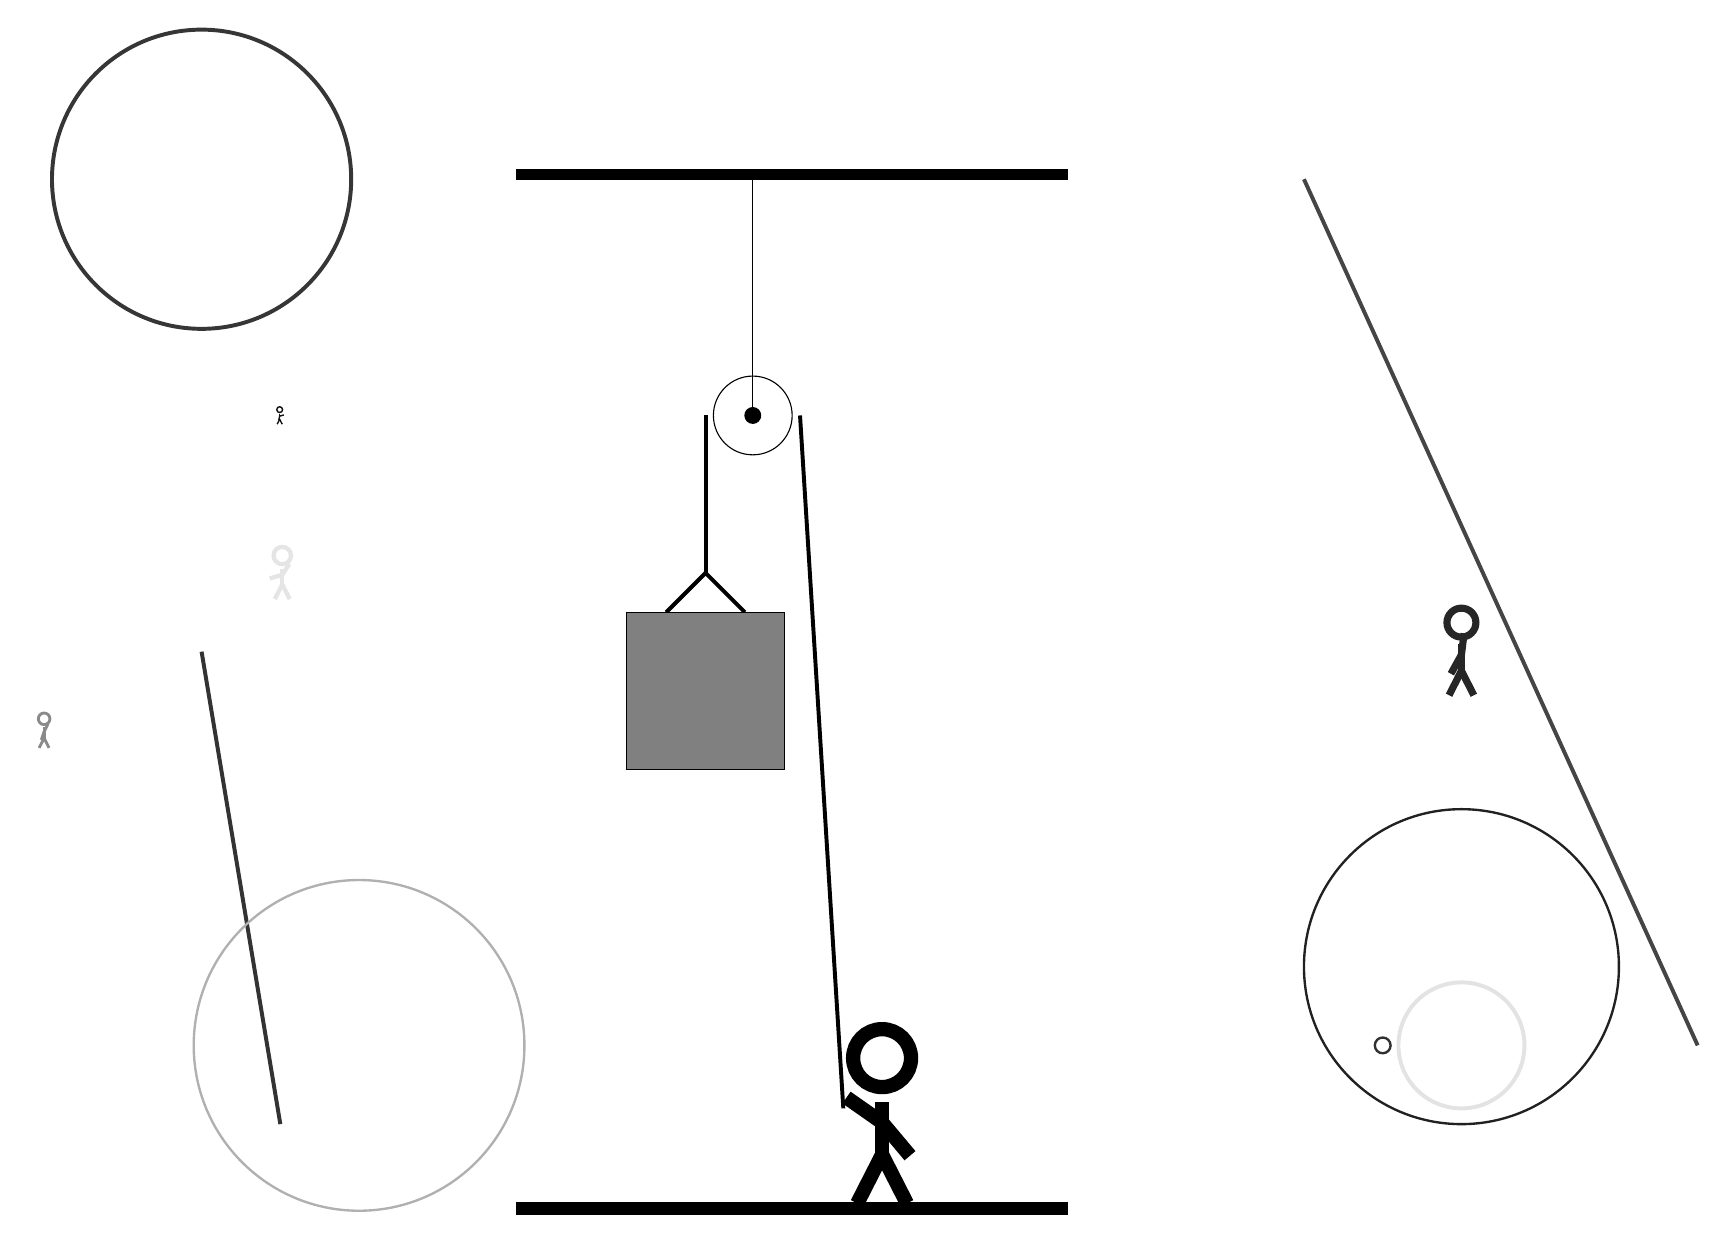
\begin{tikzpicture}
		%%%%% START %%%%%
		
		\draw[fill=black] (-2, 10) rectangle (5, 10.125);
		
		\draw (1, 7) circle (0.5);
		\draw[fill=black] (1, 7) circle (0.1);
		\draw (1, 10) -- (1, 7);
		
		\draw[line width=0.5mm] (-0.1, 4.5) -- (0.4, 5.0) -- (0.9, 4.5);
		\draw[fill=black!50] (-0.6, 4.5) rectangle (1.4, 2.5);
		
		\draw [line width=0.5mm, color=black!11](10, -1) circle (0.8);
		
		\draw [line width=0.5mm, color=black!79](-6, 10) circle (1.9);
		\draw [line width=0.3mm, color=black!81](9, -1) circle (0.1);
		\node[line width=0.3mm, color=black!10] at (-5, 5) {\Strichmaxerl[3][16][57]};
		
		\draw[line width=0.5mm, color=black!80](-6, 4) -- (-5, -2);
		\draw [line width=0.3mm, color=black!31](-4, -1) circle (2.1);
		\draw [line width=0.3mm, color=black!87](10, 0) circle (2.0);
		\node[line width=0.6mm, color=black!85] at (10, 4) {\Strichmaxerl[5][61][83]};
		\draw[line width=0.5mm, color=black!73](8, 10) -- (13, -1);
		\node[line width=0.6mm, color=black!46] at (-8, 3) {\Strichmaxerl[2][71][63]};
		
		\node[line width=0.4mm, color=black!93] at (-5, 7) {\Strichmaxerl[1][78][15]};
		
		
		\draw[line width=0.5mm] (0.4, 7) -- (0.4, 5.0);
		\centerarc[line width=0.5mm](1, 7)(0:180:0.6);
		\draw[line width=0.5mm](1.6, 7) -- (2.15, -1.8);
		
		\node at (2.6, -1.9) {\Strichmaxerl[10][-35][-50]};
		
		\draw[fill=black] (-2, -3) rectangle (5, -3.15);
		
		%%%%% END %%%%%
	\end{tikzpicture}
\end{document}